\begin{figure}[t]
\centering
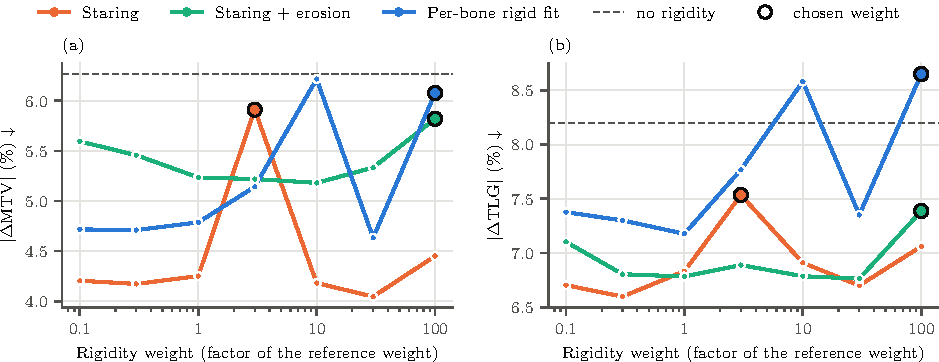
\includegraphics[width=\textwidth]{figures/rigidity_preservation.pdf}
\caption{Effect of bone-rigidity weight on lesion preservation on the validation set (26 patients, 32 lesion-positive pairs): network trained with the PET-preservation losses, followed by instance optimization (IO) with the PET-preservation terms and one bone-rigidity penalty at $0.1$ to $100$ times its calibrated reference weight.
(a)~Absolute metabolic tumor volume (MTV) change; (b)~absolute total lesion glycolysis (TLG) change.
Color identifies the bone-rigidity penalty.
Star and dashed line: IO without bone rigidity (weight 0); dotted segment: connection to the smallest nonzero weight; outlined marker: weight chosen for the test set.
Points are means over patients after averaging each patient's lesion-positive pairs.}
\label{fig:rigidity_preservation}
\end{figure}
